% Generated by paper/src/render.py from main_text.py; edit the source, not this file.
\documentclass[10pt,twocolumn]{article}
\usepackage[a4paper,margin=1.8cm,columnsep=0.7cm]{geometry}
\usepackage[T1]{fontenc}
\usepackage{lmodern}
\usepackage{microtype}
\usepackage{amsmath,amssymb}
\usepackage{booktabs}
\usepackage{array}
\usepackage{longtable}
\usepackage{graphicx}
\usepackage{caption}
\captionsetup{font=small,labelfont=bf}
\usepackage{xcolor}
\usepackage{tikz}
\usepackage[round]{natbib}
\usepackage[hidelinks]{hyperref}
\usepackage{url}
\newcommand{\dinara}{dinara-align}
\tikzset{
  dinara/.style={very thick, black},
  apafull/.style={thick, blue!80!black},
  apasimple/.style={thick, cyan!70!black, dashed},
  apa/.style={thick, violet, dotted},
  edlib/.style={thick, orange!85!black},
  biwfa/.style={thick, red!75!black, dashed},
  wfa/.style={thick, green!50!black},
}

\begin{document}
\twocolumn[
\begin{@twocolumnfalse}
{\small\textit{Bioinformatics}, Original Paper, Sequence analysis --- draft}\par\medskip
{\LARGE\bfseries dinara-align: hardware-aware algorithms for exact pairwise alignment\par}\medskip
{\large Konstantinos Kyriakidis$^{1,*}$ and Benedict Paten$^{1,*}$}\par
{\small $^{1}$UC Santa Cruz Genomics Institute, Santa Cruz, CA, USA}\par
{\small $^{*}$To whom correspondence should be addressed: kkyriaki@ucsc.edu, bpaten@ucsc.edu}\par\bigskip
\fbox{\begin{minipage}{0.97\textwidth}\small
\noindent\textbf{Motivation:} Exact pairwise alignment of long sequencing reads remains computationally demanding. Band doubling over bit-parallel blocks, the wavefront algorithm and A* with seed heuristics have greatly reduced the number of cells an exact aligner must compute. A large part of the remaining running time depends on how the computation maps onto the processor: loop-carried dependency chains, memory-bound table lookups, and bounds and thresholds that are poorly matched to the input or the hardware.\par
\noindent\textbf{Results:} We present dinara-align, an exact pairwise aligner built on algorithmic changes that address these bottlenecks: a direct construction of the neighbours of exact seed matches that provably preserves local pruning, diagonal transition vectorised across diagonals, band bounds accepted only when independent estimates agree, and per-pair optimality certificates for banded inter-sequence batches, together with a bit-parallel sweep arranged for instruction latency. On an Intel Skylake-X processor, dinara-align had the lowest mean running time among the exact aligners tested in 33 of the 34 configurations of the A*PA2 benchmark, aligning ultra-long nanopore reads in 104~ms on average, compared with 176~ms for A*PA2-full. It was 1.7 to 3.2 times faster than WFA at gap-affine costs and computed global scores for 500{,}000 short-read pairs on one core 4.5 times faster than WFA2-lib.\par
\noindent\textbf{Availability and implementation:} dinara-align is free software under the Mozilla Public License 2.0, available at \url{https://github.com/kokyriakidis/dinara-align} with C, C++, Python and command-line interfaces.\par
\noindent\textbf{Contact:} kkyriaki@ucsc.edu, bpaten@ucsc.edu\par
\noindent\textbf{Supplementary information:} Supplementary data are available at \emph{Bioinformatics} online.\par
\end{minipage}}
\bigskip
\end{@twocolumnfalse}
]
\section{Introduction}

Pairwise alignment determines the minimum-cost series of substitutions, insertions and deletions that transforms one sequence into another. The classical dynamic programming algorithm computes an \(n \times m\) matrix \citep{Gotoh1982}, which is practical for short reads but not for the hundreds of kilobases spanned by current nanopore reads. Heuristic methods restrict the computed region and lose the guarantee of optimality; exact methods instead avoid only those cells that provably cannot lie on an optimal path.

Three ideas underlie current exact aligners. \emph{Band doubling} computes only the diagonals that a path within a given cost bound can reach, and doubles the bound until the optimal cost lies within it \citep{Ukkonen1985}. \emph{Bit-parallelism} encodes a column of 64 cells in one machine word \citep{Myers1999bitvector}, and Edlib combines it with band doubling \citep{Sosic2017edlib}. \emph{Diagonal transition} extends the furthest-reaching paths one cost at a time, following runs of matches at no cost \citep{Ukkonen1985,Myers1986ond}; WFA generalised it to gap-affine costs \citep{MarcoSola2021wfa} and BiWFA reduced its memory to linear in the distance \citep{MarcoSola2023biwfa}. A*PA introduced A* search with a gap-chaining seed heuristic \citep{GrootKoerkamp2024astarpa}, and A*PA2 combined this heuristic with band doubling over SIMD blocks of bit-parallel words, aligning ultra-long reads up to 19 times faster than Edlib and BiWFA \citep{GrootKoerkamp2024astarpa2}. A second line of work accelerates the full dynamic program on vector hardware, using anti-diagonal \citep{Wozniak1997}, striped \citep{Farrar2007striped,Zhao2013ssw} and prefix-scan \citep{Daily2016parasail} layouts, difference recurrences \citep{Suzuki2018diff,Li2018minimap2}, adaptive blocks \citep{Liu2023blockaligner} and inter-sequence parallelism \citep{Rognes2011swipe,Rahn2018seqan}; these methods compute the full matrix or a fixed band, so their running time grows with its size rather than with the distance.

In the exact methods, a large part of the remaining running time is determined by how the computation maps onto the processor. The seed heuristic is built by scalar lookups in tables larger than the caches. Diagonal transition extends one diagonal at a time. Band doubling spends whole rounds when its bound is far from the distance. Batches of short pairs are vectorised across pairs, but each pair's full matrix is computed. And the bit-parallel sweep carries a dependency from each column to the next, so its speed is set by the latency of that chain rather than by its number of operations. Here we present dinara-align, an exact aligner whose algorithms address these bottlenecks. Our contributions are:

\begin{enumerate}
  \item \textbf{Direct neighbour construction for the seed heuristic.} The inexact neighbours of an exact seed match are inserted without search, and we prove that this preserves the outcome of local pruning (Lemma 1).
  \item \textbf{Gathered diagonal transition.} Diagonal transition and the gap-affine wavefront extend eight diagonals per step using gather instructions.
  \item \textbf{Band bounds from agreeing estimates.} A band-doubling bound is extrapolated from partial progress only when two independent estimates agree.
  \item \textbf{Certified bands for inter-sequence batches.} Each short pair is aligned in one vector lane within a narrow band whose optimality is certified per lane by a lower bound on the cost of any path that leaves it (Proposition 1), adapting the speculate-and-verify approach of the SeedEx accelerator \citep{Fujiki2020seedex} to software batches.
  \item \textbf{A latency-aware bit-parallel sweep.} On AVX-512, two staggered groups of words are interleaved, extending the instruction-level parallelism of A*PA2, and two Boolean identities shorten the loop-carried chain of Myers' step; the two are worth 4 to 5\% and 1 to 2\% on the ultra-long reads.
\end{enumerate}

\section{Methods}

\subsection{Problem definition and overview}

Let \(A=a_1\dots a_n\) be the reference and \(B=b_1\dots b_m\) the query, and let cell \((i,j)\) lie on diagonal \(j-i\). Under gap-affine costs, a mismatch costs \(x\) and a gap of \(k\) letters costs \(g(k)=o+ke\); unit costs correspond to \(x=e=1\) and \(o=0\), and two-piece costs take the minimum of two such functions \citep{Li2018minimap2}. A substitution matrix instead assigns each pair of letters a score to be maximised. We consider global, ends-free, extension and local alignment. An alignment is \emph{exact} if it is optimal under the requested costs, mode, band and cost limit; among optimal alignments, a fixed rule places indels leftmost or rightmost, so that the result does not depend on which algorithm computed the cost.

Each problem is assigned to an algorithm (Table~\ref{tab:engines}). For unit costs we follow A*PA2 \citep{GrootKoerkamp2024astarpa2}: band doubling over tiles of 256 columns of bit-parallel words, pruned by the gap-chaining seed heuristic \citep{GrootKoerkamp2024astarpa}, with a diagonal-transition traceback inside each tile; near-identical pairs are aligned by diagonal transition alone. Gap-affine costs use the bidirectional wavefront of WFA and BiWFA \citep{MarcoSola2021wfa,MarcoSola2023biwfa}. A short diagonal-transition search estimates the distance, and the estimate, the length and the cost model select the algorithm. The thresholds were set from measurements on each instruction set and are fixed at compile time (Supplementary Section S1).

\begin{table*}[t]
\caption{Algorithms in dinara-align and the changes introduced in this work.}\label{tab:engines}
\centering\footnotesize
\setlength{\tabcolsep}{4pt}
\begin{tabular}{@{}l>{\raggedright\arraybackslash}p{5.2cm}>{\raggedright\arraybackslash}p{5.2cm}@{}}
\toprule
Problem & Algorithm & Changes (section) \\
\midrule
Unit costs, long pairs & Band doubling over bit-parallel tiles with the gap-chaining seed heuristic (A*PA2) & Regrouped recurrence, staggered groups (2.2); agreeing bounds (2.3); neighbour construction (2.5) \\
Unit costs, similar pairs & Diagonal transition (WFA, BiWFA) & Gathered extension (2.4) \\
Gap-affine, two-piece & Bidirectional wavefront (WFA, BiWFA) & Gathered extension (2.4); score-derived band (2.7) \\
Substitution matrices, local & Anti-diagonal vector sweep; end-first local alignment (SSW) & Backward wavefront from the best end (2.7) \\
Batches of short pairs & Inter-sequence vectorisation (SWIPE, SeqAn, parasail) & Certified per-lane bands (2.6) \\
\bottomrule
\end{tabular}
\end{table*}

\subsection{A shorter critical path for Myers' recurrence}

As in Edlib and A*PA2 \citep{Sosic2017edlib,GrootKoerkamp2024astarpa2}, the query is packed 64 bases per word, and Myers' recurrence \citep{Myers1999bitvector} advances a word by one column. With match mask \(E\), vertical difference masks \(P_v, M_v\) and the incoming negative horizontal difference folded into \(E' = E \lor M_h^{\mathrm{in}}\), A*PA2 computes

\begin{equation}\begin{gathered}
c = (E' \land P_v) + P_v,\\ X_h = (c \oplus P_v) \lor E',\\ P_h = M_v \lor \lnot(X_h \lor P_v),\\ M_h = P_v \land X_h.
\end{gathered}\end{equation}

The horizontal masks \(P_h\) and \(M_h\) determine the vertical masks of the next column, so the path from \(c\) to them lies on the loop-carried chain. Since \((c \oplus P_v) \lor P_v = c \lor P_v\) and \(P_v \land (c \oplus P_v) = P_v \land \lnot c\), the same masks are obtained as

\begin{equation}\begin{gathered}
P_h = M_v \lor \lnot\bigl(c \lor (E' \lor P_v)\bigr),\\ M_h = (P_v \land \lnot c) \lor (P_v \land E'),
\end{gathered}\end{equation}

where \(E' \lor P_v\) and \(P_v \land E'\) do not depend on \(c\) and are computed off the critical path. This removes two operations from the loop-carried chain and, for a single word, reduces the cost from 14 to 8 cycles per column on the Skylake-X. Myers \citep{Myers1999bitvector}, Edlib and A*PA2 use the original form, and we are not aware of a previous description of the regrouped one.

Words occupy the lanes of a vector, staggered by one column, so that the horizontal difference leaving one word enters the next through a lane rotation \citep{Wozniak1997,GrootKoerkamp2024astarpa2}. Every column then waits for the rotation of the previous one, and A*PA2 processes two four-lane vectors together to overlap these waits. On AVX-512, where a vector holds eight words, dinara-align interleaves two eight-word groups, the lower lagging ten columns behind the upper, so that the instructions of each group fill the latency of the other; with narrower vectors a single group is used. Bands of two or three words, in which every operation lies on the critical path, are computed in general-purpose registers, whose operations have lower latency. On AVX-512 the sweep requires about 2.4 cycles per word and column.

\subsection{Band bounds from agreeing estimates}

Band doubling returns the exact distance for any initial bound, but its running time depends on how close that bound is to the distance. A partial computation that has reached cost \(s\) at anti-diagonal \(r\) suggests the extrapolated distance \(\hat d = s(n+m)/r\). This extrapolation is reliable when edits are spread evenly along the pair and can be too high by orders of magnitude when they are concentrated, as near the ends of nanopore reads. dinara-align therefore computes two extrapolations, \(\hat d_1\) from the first eight edits of a diagonal-transition search and \(\hat d_2\) from the same search continued until its budget, and sets the first bound from them only if \(\max(\hat d_1,\hat d_2) \le \tfrac43 \min(\hat d_1,\hat d_2)\). Otherwise, as in A*PA2, the bound starts 256 above the known lower bound and doubles. Within a round, the distance is extrapolated again after one eighth, one quarter and one half of the columns; the bound is lowered if the extrapolation lies below it, and the round is abandoned if the extrapolation exceeds it. Because these rules change only the sequence of bounds, the result remains exact.

\subsection{Gathered diagonal transition}

Diagonal transition extends each diagonal of a wavefront along its run of matches. dinara-align compares eight letters at a time by the exclusive-or of two 64-bit words and a count of trailing zeros. On AVX-512, eight diagonals are extended together: their letters are loaded with gather instructions, and the wavefront is padded with unreachable diagonals so that every step processes full vectors under branch-free masks. The gather masks are derived from the lanes of each group, which avoids a dependency between consecutive gathers that would otherwise serialise them. The same vectorised step serves near-identical pairs, computed from one or both ends \citep{MarcoSola2023biwfa}, the traceback inside each tile, restricted to the diagonals that can still reach the traced cell, and the three-layer gap-affine wavefront.

\subsection{Seed heuristic: direct neighbour construction}

The reference is divided into disjoint seeds of 12 bases, matched exactly, or of 16 bases, matched with at most one edit \citep{GrootKoerkamp2024astarpa}. A 16-base seed that matches with at most one edit matches one of its two 8-base halves exactly, so each half indexes a table. Since these tables exceed the caches, the lookups for 16 query rows are issued together, so that their memory accesses overlap, and only seeds whose matches could still chain to the end of the pair are considered.

An exact match \(\mu\) of a seed at query rows \([i, i+16)\) always has four neighbouring matches with one edit: two share its start, at rows \([i, i+15)\) and \([i, i+17)\), and two share its end, at \([i+1, i+16)\) and \([i-1, i+16)\). Because chaining is all-or-nothing, a neighbour one diagonal away may chain where \(\mu\) cannot, and the neighbours are required for the heuristic to remain a lower bound. Rather than locating them by search and testing each for local pruning, dinara-align inserts them whenever \(\mu\) is retained, which is justified by the following lemma. Local pruning retains a match \(\nu\) of a seed only if \(c(\nu) + h(e(\nu)) < \tau\), where \(c(\nu)\) is its cost, \(e(\nu)\) its end cell, \(h(u)\) the least cost of a path from \(u\) across the following seeds, and \(\tau\) a threshold that depends only on the seeds.

\textbf{Lemma 1.} If an exact match \(\mu\) fails local pruning, so does each of its four neighbours.

\emph{Proof.} A neighbour \(\nu\) that shares the end of \(\mu\) has \(e(\nu)=e(\mu)\) and \(c(\nu)=1>c(\mu)=0\). A neighbour that shares the start ends on an adjacent diagonal, and one insertion or deletion from \(e(\mu)\) reaches a cell on that diagonal at or beyond \(e(\nu)\). The least remaining cost does not increase along a diagonal \citep{Ukkonen1985}, so \(h(e(\mu)) \le 1 + h(e(\nu))\) and \(c(\mu)+h(e(\mu)) \le c(\nu)+h(e(\nu))\). In both cases the pruning test value of \(\nu\) is at least that of \(\mu\). \(\square\)

Neighbours sharing the start therefore raise the layer of that start by the chain length available from their ends, and neighbours sharing the end are placed one layer below it, without a search or a pruning test of their own.

\subsection{Certified bands for inter-sequence batches}

Batches of short pairs are aligned with one pair per vector lane \citep{Rognes2011swipe,Rahn2018seqan}, first in saturating 8-bit lanes and, for pairs that saturate, in 16-bit lanes \citep{Zhao2013ssw,Daily2016parasail}. Rather than computing each matrix in full, a lane computes the band of diagonals \([d_\ell, d_h]\) containing the main diagonal 0 and the end diagonal \(\delta = m - n\), together with one further diagonal on either side. Its optimality is certified with the following bound, a cost form of the out-of-band bounds of \citet{Gibrat2018band} and \citet{Fujiki2020seedex}, stated for gap-affine and two-piece costs and with a strict form for tie-breaking.

\textbf{Proposition 1.} Let \(C\) be the least cost of an alignment within \([d_\ell, d_h]\), and let \(L(d) = g(|d|) + g(|d-\delta|)\). If \(C \le \min\bigl(L(d_h+1), L(d_\ell-1)\bigr)\), then \(C\) is the optimal cost; if the inequality is strict, every optimal alignment lies within the band.

\emph{Proof.} An alignment that leaves the band visits diagonal \(d_h+1\) or \(d_\ell-1\). Consider \(d=d_h+1 > \max(0,\delta)\); the case below the band is symmetric. Starting on diagonal 0, the alignment contains insertions totalling at least \(d\) letters to reach \(d\), and deletions totalling at least \(d-\delta\) letters to end on \(\delta\). These form at least one gap of each kind, and since \(g\) is subadditive (for two-piece costs, with the usual convention that the longer piece has the lower extension cost), their total cost is at least \(g(d)+g(d-\delta)=L(d)\). Every alignment outside the band therefore costs at least \(\min\bigl(L(d_h+1), L(d_\ell-1)\bigr)\). \(\square\)

Bounds of this kind underlie band doubling \citep{Ukkonen1985} and have been used to verify narrow-band results in software \citep{Gibrat2018band} and in hardware \citep{Fujiki2020seedex}; here the certificate is evaluated independently in each vector lane of an inter-sequence batch. For alignments, the strict form guarantees that the alignment selected by the tie rule lies within the band. Pairs that fail the certificate, about one in seven in our short-read benchmark, are recomputed over every diagonal that a cheaper path could visit, grouped by the width of that band so that the lanes of a group finish together.

\subsection{Gap-affine and score-based alignment}

A scoring scheme with match score \(a\), mismatch score \(b\) and gap scores \(-(o+ke)\) can be converted into costs for global alignment \citep{Eizenga2022wfalm}. Every alignment covers \(n+m\) letters, so its score \(S\) and a gap-affine cost \(C\) satisfy

\begin{equation}\begin{gathered}
S = \tfrac12\bigl(a(n+m) - C\bigr),\\ C = 2(a-b)\,X + \sum_{\text{gaps}} \bigl(2o + k(2e+a)\bigr),
\end{gathered}\end{equation}

where \(X\) is the number of mismatches, so the wavefront computes score-maximising alignments. The cost also bounds the band in which the alignment must be stored. Each gapped letter contributes at least \(2e+a\) to \(C\), and an alignment that deviates by \(t\) diagonals from both the main and the end diagonal contains at least \(2t\) gapped letters; hence only diagonals within \(C/(2(2e+a))\) of them can contain an optimal alignment. For a 1~kbp pair at 5\% divergence, this stores 137 diagonals instead of 1{,}000. Under a general substitution matrix, anti-diagonals are computed in 16-bit vector lanes while the scores provably fit \citep{Wozniak1997}. Local alignment first locates the end of the optimal alignment with a forward sweep, as in SSW \citep{Zhao2013ssw}, and then extends a wavefront backwards from that end, stopping at the first cell that attains the maximal score; this avoids the correction pass that striped layouts may need when long alignments score highly \citep{Farrar2007striped}.

\subsection{Validation}

A differential fuzzer compares results for random pairs, cost models, modes, bands, cost limits and tie-breaking rules with a full-matrix reference implementation that shares no code with the library, checking validity, optimality, the symmetry of the two tie-breaking rules and agreement between batched and single calls. The WFA2-lib regression set is reproduced exactly, including all CIGAR strings under the rightmost tie-breaking rule. The seed heuristic is compared with the true remaining cost at every cell of random pairs; this check found and confirmed the correction of an implementation error that caused occasional overestimates (Supplementary Section S1).

\section{Results}

\subsection{Experimental setup}

All measurements were taken on an Intel Core i9-7900X (Skylake-X, AVX-512) with ten cores fixed at 3.3~GHz, turbo boost and hyper-threading disabled, and 91~GB of memory, running Ubuntu 26.04. dinara-align is implemented in Mojo \citep{Modular2025mojo} and was compiled with Mojo 1.1.0 at commit \texttt{ebe290f}; all tools were compiled for the native instruction set. The exact aligners compared are A*PA2-full and A*PA2-simple \citep{GrootKoerkamp2024astarpa2}, A*PA \citep{GrootKoerkamp2024astarpa}, Edlib \citep{Sosic2017edlib}, WFA and BiWFA \citep{MarcoSola2021wfa,MarcoSola2023biwfa}, KSW2 \citep{Li2018minimap2,Suzuki2018diff}, parasail \citep{Daily2016parasail}, SSW \citep{Zhao2013ssw}, abPOA \citep{Gao2021abpoa} and hyalite \citep{hyalite}. Every cost was compared with those of every other tool and with the costs recorded in the published A*PA2 results; no discrepancies occurred.

For unit costs we followed the A*PA2 protocol \citep{GrootKoerkamp2024astarpa2}: one single-threaded job at a time, pinned to one core, each pair aligned once with traceback, and a time limit of 20~s per sample, after which only the completed pairs are reported. The datasets are those of A*PA2: nanopore reads of about 1, 10 and 50~kbp, ultra-long reads over 500~kbp with and without genetic variation, SARS-CoV-2 genomes, and uniform-error pairs regenerated from the original random seed. We report the mean wall-clock time per alignment, excluding input, and the increase in peak resident memory during an alignment, measured with \texttt{getrusage}. As in A*PA2, each sample was run once; the one configuration in which dinara-align was not the fastest was repeated five times. Other workloads were timed in-process after a warm-up, as the fastest of twenty batches of about 10~ms, or once for calls of 0.1~s or longer; short-read batches as the faster of two passes.

\subsection{Edit distance}

On the real datasets, dinara-align had the lowest mean and median time among the exact aligners (Table~\ref{tab:real}; Supplementary Table S4). It aligned the 1~kbp reads in 23~\textmu s, compared with 31~\textmu s for WFA, required about two thirds of the time of A*PA2-simple on the 10 and 50~kbp reads, and aligned the ultra-long reads in 104 and 144~ms, compared with 176 and 210~ms for A*PA2-full. The approximate aligners WFA-adaptive \citep{MarcoSola2021wfa} and Block Aligner \citep{Liu2023blockaligner} were slower than dinara-align on every dataset.

\begin{table*}[t]
\caption{Unit-cost alignment of the A*PA2 real datasets: mean time per alignment, traceback included. Superscripts give the number of pairs completed within 20~s where not all were; a dash marks a tool that completed none.}\label{tab:real}
\centering\footnotesize
\setlength{\tabcolsep}{4pt}
\begin{tabular}{@{}lrrrrrrr@{}}
\toprule
Dataset & dinara-align & A*PA2-full & A*PA2-simple & A*PA & Edlib & BiWFA & WFA \\
\midrule
ont-1k (0.8~kbp) & \textbf{23~\textmu s} & 81~\textmu s & 48~\textmu s & 612~\textmu s & 126~\textmu s & 44~\textmu s & 31~\textmu s \\
ont-10k (3.6~kbp) & \textbf{163~\textmu s} & 391~\textmu s & 247~\textmu s & 15.3~ms & 1.1~ms & 753~\textmu s & 595~\textmu s \\
ont-50k (9.5~kbp) & \textbf{587~\textmu s} & 1.27~ms & 944~\textmu s & 190~ms$^{81/104}$ & 6.1~ms & 7.43~ms & 6.37~ms \\
ont-500k (638~kbp) & \textbf{104~ms} & 176~ms & 537~ms & – & 4.99~s$^{4/15}$ & 19.8~s$^{1/15}$ & – \\
genvar (651~kbp) & \textbf{144~ms} & 210~ms & 624~ms & – & 5.23~s$^{4/15}$ & 6.36~s$^{3/15}$ & – \\
SARS-CoV-2 (30~kbp) & \textbf{279~\textmu s} & 2.00~ms & 728~\textmu s & 6.49~ms & 8.15~ms & 895~\textmu s & 983~\textmu s \\
\bottomrule
\end{tabular}
\end{table*}

On uniform 100~kbp pairs (Fig.~\ref{fig:sweeps}a), dinara-align required 4.4 to 6.8~ms between 2 and 8\% divergence and 10.4 to 12.3~ms from 9 to 15\%, where A*PA2-full required up to 18~ms. A*PA2-full was faster only at 10\% divergence (10.5 versus 11.0~ms; in five repeated runs, 10.43–10.49 versus 11.02–11.06~ms). With increasing length (Fig.~\ref{fig:sweeps}b), dinara-align aligned 1~Mbp pairs at 15\% divergence in 265~ms, compared with 1.33~s for A*PA2-full and 2.07~s for A*PA.

\begin{figure*}[t]
\centering
\begin{minipage}{0.49\textwidth}\centering\textbf{a}\par\resizebox{\linewidth}{!}{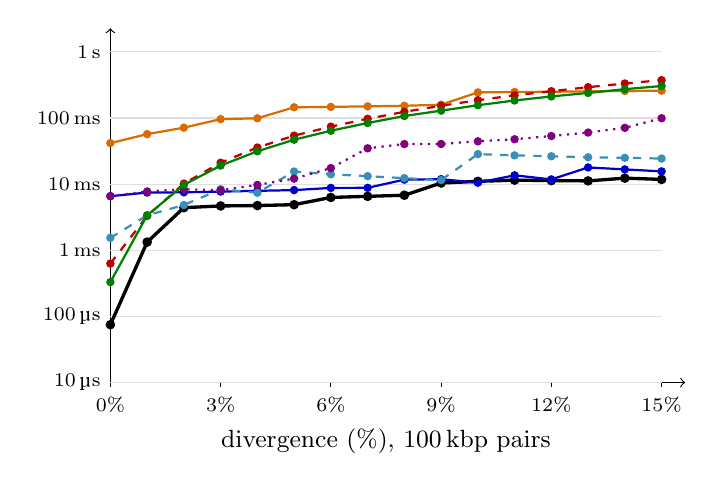
\begin{tikzpicture}
\draw[->] (0,0) -- (7.30,0);
\draw[->] (0,0) -- (0,4.50);
\draw[gray!25] (0,0.000) -- (7.00,0.000); \node[left,font=\scriptsize] at (0,0.000) {10\,\textmu s};
\draw[gray!25] (0,0.840) -- (7.00,0.840); \node[left,font=\scriptsize] at (0,0.840) {100\,\textmu s};
\draw[gray!25] (0,1.680) -- (7.00,1.680); \node[left,font=\scriptsize] at (0,1.680) {1\,ms};
\draw[gray!25] (0,2.520) -- (7.00,2.520); \node[left,font=\scriptsize] at (0,2.520) {10\,ms};
\draw[gray!25] (0,3.360) -- (7.00,3.360); \node[left,font=\scriptsize] at (0,3.360) {100\,ms};
\draw[gray!25] (0,4.200) -- (7.00,4.200); \node[left,font=\scriptsize] at (0,4.200) {1\,s};
\draw (0.000,0) -- (0.000,-0.06) node[below,font=\scriptsize] {0\%};
\draw (1.400,0) -- (1.400,-0.06) node[below,font=\scriptsize] {3\%};
\draw (2.800,0) -- (2.800,-0.06) node[below,font=\scriptsize] {6\%};
\draw (4.200,0) -- (4.200,-0.06) node[below,font=\scriptsize] {9\%};
\draw (5.600,0) -- (5.600,-0.06) node[below,font=\scriptsize] {12\%};
\draw (7.000,0) -- (7.000,-0.06) node[below,font=\scriptsize] {15\%};
\node[font=\small] at (3.50,-0.75) {divergence (\%), 100\,kbp pairs};
\draw[dinara] plot coordinates {(0.000,0.735) (0.467,1.784) (0.933,2.221) (1.400,2.243) (1.867,2.248) (2.333,2.259) (2.800,2.351) (3.267,2.365) (3.733,2.379) (4.200,2.534) (4.667,2.555) (5.133,2.571) (5.600,2.565) (6.067,2.561) (6.533,2.596) (7.000,2.580)};
\draw[dinara,solid,fill=.] (0.000,0.735) circle (1.1pt);
\draw[dinara,solid,fill=.] (0.467,1.784) circle (1.1pt);
\draw[dinara,solid,fill=.] (0.933,2.221) circle (1.1pt);
\draw[dinara,solid,fill=.] (1.400,2.243) circle (1.1pt);
\draw[dinara,solid,fill=.] (1.867,2.248) circle (1.1pt);
\draw[dinara,solid,fill=.] (2.333,2.259) circle (1.1pt);
\draw[dinara,solid,fill=.] (2.800,2.351) circle (1.1pt);
\draw[dinara,solid,fill=.] (3.267,2.365) circle (1.1pt);
\draw[dinara,solid,fill=.] (3.733,2.379) circle (1.1pt);
\draw[dinara,solid,fill=.] (4.200,2.534) circle (1.1pt);
\draw[dinara,solid,fill=.] (4.667,2.555) circle (1.1pt);
\draw[dinara,solid,fill=.] (5.133,2.571) circle (1.1pt);
\draw[dinara,solid,fill=.] (5.600,2.565) circle (1.1pt);
\draw[dinara,solid,fill=.] (6.067,2.561) circle (1.1pt);
\draw[dinara,solid,fill=.] (6.533,2.596) circle (1.1pt);
\draw[dinara,solid,fill=.] (7.000,2.580) circle (1.1pt);
\draw[apafull] plot coordinates {(0.000,2.367) (0.467,2.413) (0.933,2.416) (1.400,2.425) (1.867,2.435) (2.333,2.444) (2.800,2.472) (3.267,2.473) (3.733,2.577) (4.200,2.583) (4.667,2.538) (5.133,2.632) (5.600,2.580) (6.067,2.732) (6.533,2.707) (7.000,2.682)};
\draw[apafull,solid,fill=.] (0.000,2.367) circle (1.1pt);
\draw[apafull,solid,fill=.] (0.467,2.413) circle (1.1pt);
\draw[apafull,solid,fill=.] (0.933,2.416) circle (1.1pt);
\draw[apafull,solid,fill=.] (1.400,2.425) circle (1.1pt);
\draw[apafull,solid,fill=.] (1.867,2.435) circle (1.1pt);
\draw[apafull,solid,fill=.] (2.333,2.444) circle (1.1pt);
\draw[apafull,solid,fill=.] (2.800,2.472) circle (1.1pt);
\draw[apafull,solid,fill=.] (3.267,2.473) circle (1.1pt);
\draw[apafull,solid,fill=.] (3.733,2.577) circle (1.1pt);
\draw[apafull,solid,fill=.] (4.200,2.583) circle (1.1pt);
\draw[apafull,solid,fill=.] (4.667,2.538) circle (1.1pt);
\draw[apafull,solid,fill=.] (5.133,2.632) circle (1.1pt);
\draw[apafull,solid,fill=.] (5.600,2.580) circle (1.1pt);
\draw[apafull,solid,fill=.] (6.067,2.732) circle (1.1pt);
\draw[apafull,solid,fill=.] (6.533,2.707) circle (1.1pt);
\draw[apafull,solid,fill=.] (7.000,2.682) circle (1.1pt);
\draw[apasimple] plot coordinates {(0.000,1.838) (0.467,2.124) (0.933,2.255) (1.400,2.455) (1.867,2.410) (2.333,2.680) (2.800,2.645) (3.267,2.621) (3.733,2.596) (4.200,2.571) (4.667,2.901) (5.133,2.885) (5.600,2.874) (6.067,2.861) (6.533,2.854) (7.000,2.845)};
\draw[apasimple,solid,fill=.] (0.000,1.838) circle (1.1pt);
\draw[apasimple,solid,fill=.] (0.467,2.124) circle (1.1pt);
\draw[apasimple,solid,fill=.] (0.933,2.255) circle (1.1pt);
\draw[apasimple,solid,fill=.] (1.400,2.455) circle (1.1pt);
\draw[apasimple,solid,fill=.] (1.867,2.410) circle (1.1pt);
\draw[apasimple,solid,fill=.] (2.333,2.680) circle (1.1pt);
\draw[apasimple,solid,fill=.] (2.800,2.645) circle (1.1pt);
\draw[apasimple,solid,fill=.] (3.267,2.621) circle (1.1pt);
\draw[apasimple,solid,fill=.] (3.733,2.596) circle (1.1pt);
\draw[apasimple,solid,fill=.] (4.200,2.571) circle (1.1pt);
\draw[apasimple,solid,fill=.] (4.667,2.901) circle (1.1pt);
\draw[apasimple,solid,fill=.] (5.133,2.885) circle (1.1pt);
\draw[apasimple,solid,fill=.] (5.600,2.874) circle (1.1pt);
\draw[apasimple,solid,fill=.] (6.067,2.861) circle (1.1pt);
\draw[apasimple,solid,fill=.] (6.533,2.854) circle (1.1pt);
\draw[apasimple,solid,fill=.] (7.000,2.845) circle (1.1pt);
\draw[apa] plot coordinates {(0.000,2.367) (0.467,2.427) (0.933,2.455) (1.400,2.442) (1.867,2.510) (2.333,2.590) (2.800,2.724) (3.267,2.975) (3.733,3.029) (4.200,3.030) (4.667,3.064) (5.133,3.090) (5.600,3.131) (6.067,3.175) (6.533,3.235) (7.000,3.357)};
\draw[apa,solid,fill=.] (0.000,2.367) circle (1.1pt);
\draw[apa,solid,fill=.] (0.467,2.427) circle (1.1pt);
\draw[apa,solid,fill=.] (0.933,2.455) circle (1.1pt);
\draw[apa,solid,fill=.] (1.400,2.442) circle (1.1pt);
\draw[apa,solid,fill=.] (1.867,2.510) circle (1.1pt);
\draw[apa,solid,fill=.] (2.333,2.590) circle (1.1pt);
\draw[apa,solid,fill=.] (2.800,2.724) circle (1.1pt);
\draw[apa,solid,fill=.] (3.267,2.975) circle (1.1pt);
\draw[apa,solid,fill=.] (3.733,3.029) circle (1.1pt);
\draw[apa,solid,fill=.] (4.200,3.030) circle (1.1pt);
\draw[apa,solid,fill=.] (4.667,3.064) circle (1.1pt);
\draw[apa,solid,fill=.] (5.133,3.090) circle (1.1pt);
\draw[apa,solid,fill=.] (5.600,3.131) circle (1.1pt);
\draw[apa,solid,fill=.] (6.067,3.175) circle (1.1pt);
\draw[apa,solid,fill=.] (6.533,3.235) circle (1.1pt);
\draw[apa,solid,fill=.] (7.000,3.357) circle (1.1pt);
\draw[edlib] plot coordinates {(0.000,3.041) (0.467,3.155) (0.933,3.237) (1.400,3.345) (1.867,3.356) (2.333,3.496) (2.800,3.501) (3.267,3.508) (3.733,3.515) (4.200,3.529) (4.667,3.685) (5.133,3.690) (5.600,3.693) (6.067,3.699) (6.533,3.703) (7.000,3.707)};
\draw[edlib,solid,fill=.] (0.000,3.041) circle (1.1pt);
\draw[edlib,solid,fill=.] (0.467,3.155) circle (1.1pt);
\draw[edlib,solid,fill=.] (0.933,3.237) circle (1.1pt);
\draw[edlib,solid,fill=.] (1.400,3.345) circle (1.1pt);
\draw[edlib,solid,fill=.] (1.867,3.356) circle (1.1pt);
\draw[edlib,solid,fill=.] (2.333,3.496) circle (1.1pt);
\draw[edlib,solid,fill=.] (2.800,3.501) circle (1.1pt);
\draw[edlib,solid,fill=.] (3.267,3.508) circle (1.1pt);
\draw[edlib,solid,fill=.] (3.733,3.515) circle (1.1pt);
\draw[edlib,solid,fill=.] (4.200,3.529) circle (1.1pt);
\draw[edlib,solid,fill=.] (4.667,3.685) circle (1.1pt);
\draw[edlib,solid,fill=.] (5.133,3.690) circle (1.1pt);
\draw[edlib,solid,fill=.] (5.600,3.693) circle (1.1pt);
\draw[edlib,solid,fill=.] (6.067,3.699) circle (1.1pt);
\draw[edlib,solid,fill=.] (6.533,3.703) circle (1.1pt);
\draw[edlib,solid,fill=.] (7.000,3.707) circle (1.1pt);
\draw[biwfa] plot coordinates {(0.000,1.511) (0.467,2.116) (0.933,2.527) (1.400,2.792) (1.867,2.985) (2.333,3.136) (2.800,3.250) (3.267,3.350) (3.733,3.438) (4.200,3.515) (4.667,3.586) (5.133,3.648) (5.600,3.700) (6.067,3.751) (6.533,3.798) (7.000,3.841)};
\draw[biwfa,solid,fill=.] (0.000,1.511) circle (1.1pt);
\draw[biwfa,solid,fill=.] (0.467,2.116) circle (1.1pt);
\draw[biwfa,solid,fill=.] (0.933,2.527) circle (1.1pt);
\draw[biwfa,solid,fill=.] (1.400,2.792) circle (1.1pt);
\draw[biwfa,solid,fill=.] (1.867,2.985) circle (1.1pt);
\draw[biwfa,solid,fill=.] (2.333,3.136) circle (1.1pt);
\draw[biwfa,solid,fill=.] (2.800,3.250) circle (1.1pt);
\draw[biwfa,solid,fill=.] (3.267,3.350) circle (1.1pt);
\draw[biwfa,solid,fill=.] (3.733,3.438) circle (1.1pt);
\draw[biwfa,solid,fill=.] (4.200,3.515) circle (1.1pt);
\draw[biwfa,solid,fill=.] (4.667,3.586) circle (1.1pt);
\draw[biwfa,solid,fill=.] (5.133,3.648) circle (1.1pt);
\draw[biwfa,solid,fill=.] (5.600,3.700) circle (1.1pt);
\draw[biwfa,solid,fill=.] (6.067,3.751) circle (1.1pt);
\draw[biwfa,solid,fill=.] (6.533,3.798) circle (1.1pt);
\draw[biwfa,solid,fill=.] (7.000,3.841) circle (1.1pt);
\draw[wfa] plot coordinates {(0.000,1.276) (0.467,2.124) (0.933,2.510) (1.400,2.756) (1.867,2.937) (2.333,3.084) (2.800,3.198) (3.267,3.296) (3.733,3.385) (4.200,3.453) (4.667,3.522) (5.133,3.582) (5.600,3.634) (6.067,3.678) (6.533,3.726) (7.000,3.766)};
\draw[wfa,solid,fill=.] (0.000,1.276) circle (1.1pt);
\draw[wfa,solid,fill=.] (0.467,2.124) circle (1.1pt);
\draw[wfa,solid,fill=.] (0.933,2.510) circle (1.1pt);
\draw[wfa,solid,fill=.] (1.400,2.756) circle (1.1pt);
\draw[wfa,solid,fill=.] (1.867,2.937) circle (1.1pt);
\draw[wfa,solid,fill=.] (2.333,3.084) circle (1.1pt);
\draw[wfa,solid,fill=.] (2.800,3.198) circle (1.1pt);
\draw[wfa,solid,fill=.] (3.267,3.296) circle (1.1pt);
\draw[wfa,solid,fill=.] (3.733,3.385) circle (1.1pt);
\draw[wfa,solid,fill=.] (4.200,3.453) circle (1.1pt);
\draw[wfa,solid,fill=.] (4.667,3.522) circle (1.1pt);
\draw[wfa,solid,fill=.] (5.133,3.582) circle (1.1pt);
\draw[wfa,solid,fill=.] (5.600,3.634) circle (1.1pt);
\draw[wfa,solid,fill=.] (6.067,3.678) circle (1.1pt);
\draw[wfa,solid,fill=.] (6.533,3.726) circle (1.1pt);
\draw[wfa,solid,fill=.] (7.000,3.766) circle (1.1pt);
\end{tikzpicture}}\end{minipage}\hfill\begin{minipage}{0.49\textwidth}\centering\textbf{b}\par\resizebox{\linewidth}{!}{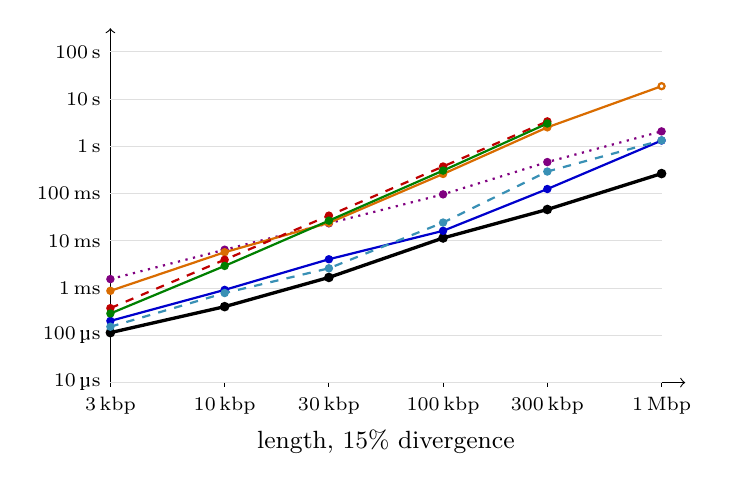
\begin{tikzpicture}
\draw[->] (0,0) -- (7.30,0);
\draw[->] (0,0) -- (0,4.50);
\draw[gray!25] (0,0.000) -- (7.00,0.000); \node[left,font=\scriptsize] at (0,0.000) {10\,\textmu s};
\draw[gray!25] (0,0.600) -- (7.00,0.600); \node[left,font=\scriptsize] at (0,0.600) {100\,\textmu s};
\draw[gray!25] (0,1.200) -- (7.00,1.200); \node[left,font=\scriptsize] at (0,1.200) {1\,ms};
\draw[gray!25] (0,1.800) -- (7.00,1.800); \node[left,font=\scriptsize] at (0,1.800) {10\,ms};
\draw[gray!25] (0,2.400) -- (7.00,2.400); \node[left,font=\scriptsize] at (0,2.400) {100\,ms};
\draw[gray!25] (0,3.000) -- (7.00,3.000); \node[left,font=\scriptsize] at (0,3.000) {1\,s};
\draw[gray!25] (0,3.600) -- (7.00,3.600); \node[left,font=\scriptsize] at (0,3.600) {10\,s};
\draw[gray!25] (0,4.200) -- (7.00,4.200); \node[left,font=\scriptsize] at (0,4.200) {100\,s};
\draw (0.000,0) -- (0.000,-0.06) node[below,font=\scriptsize] {3\,kbp};
\draw (1.451,0) -- (1.451,-0.06) node[below,font=\scriptsize] {10\,kbp};
\draw (2.775,0) -- (2.775,-0.06) node[below,font=\scriptsize] {30\,kbp};
\draw (4.225,0) -- (4.225,-0.06) node[below,font=\scriptsize] {100\,kbp};
\draw (5.549,0) -- (5.549,-0.06) node[below,font=\scriptsize] {300\,kbp};
\draw (7.000,0) -- (7.000,-0.06) node[below,font=\scriptsize] {1\,Mbp};
\node[font=\small] at (3.50,-0.75) {length, 15\% divergence};
\draw[dinara] plot coordinates {(0.000,0.634) (1.451,0.964) (2.775,1.335) (4.225,1.836) (5.549,2.198) (7.000,2.654)};
\draw[dinara,solid,fill=.] (0.000,0.634) circle (1.1pt);
\draw[dinara,solid,fill=.] (1.451,0.964) circle (1.1pt);
\draw[dinara,solid,fill=.] (2.775,1.335) circle (1.1pt);
\draw[dinara,solid,fill=.] (4.225,1.836) circle (1.1pt);
\draw[dinara,solid,fill=.] (5.549,2.198) circle (1.1pt);
\draw[dinara,solid,fill=.] (7.000,2.654) circle (1.1pt);
\draw[apafull] plot coordinates {(0.000,0.783) (1.451,1.177) (2.775,1.566) (4.225,1.927) (5.549,2.458) (7.000,3.074)};
\draw[apafull,solid,fill=.] (0.000,0.783) circle (1.1pt);
\draw[apafull,solid,fill=.] (1.451,1.177) circle (1.1pt);
\draw[apafull,solid,fill=.] (2.775,1.566) circle (1.1pt);
\draw[apafull,solid,fill=.] (4.225,1.927) circle (1.1pt);
\draw[apafull,solid,fill=.] (5.549,2.458) circle (1.1pt);
\draw[apafull,solid,fill=.] (7.000,3.074) circle (1.1pt);
\draw[apasimple] plot coordinates {(0.000,0.709) (1.451,1.137) (2.775,1.451) (4.225,2.032) (5.549,2.680) (7.000,3.076)};
\draw[apasimple,solid,fill=.] (0.000,0.709) circle (1.1pt);
\draw[apasimple,solid,fill=.] (1.451,1.137) circle (1.1pt);
\draw[apasimple,solid,fill=.] (2.775,1.451) circle (1.1pt);
\draw[apasimple,solid,fill=.] (4.225,2.032) circle (1.1pt);
\draw[apasimple,solid,fill=.] (5.549,2.680) circle (1.1pt);
\draw[apasimple,solid,fill=.] (7.000,3.076) circle (1.1pt);
\draw[apa] plot coordinates {(0.000,1.314) (1.451,1.687) (2.775,2.022) (4.225,2.390) (5.549,2.800) (7.000,3.190)};
\draw[apa,solid,fill=.] (0.000,1.314) circle (1.1pt);
\draw[apa,solid,fill=.] (1.451,1.687) circle (1.1pt);
\draw[apa,solid,fill=.] (2.775,2.022) circle (1.1pt);
\draw[apa,solid,fill=.] (4.225,2.390) circle (1.1pt);
\draw[apa,solid,fill=.] (5.549,2.800) circle (1.1pt);
\draw[apa,solid,fill=.] (7.000,3.190) circle (1.1pt);
\draw[edlib] plot coordinates {(0.000,1.165) (1.451,1.655) (2.775,2.028) (4.225,2.649) (5.549,3.241) (7.000,3.764)};
\draw[edlib,solid,fill=.] (0.000,1.165) circle (1.1pt);
\draw[edlib,solid,fill=.] (1.451,1.655) circle (1.1pt);
\draw[edlib,solid,fill=.] (2.775,2.028) circle (1.1pt);
\draw[edlib,solid,fill=.] (4.225,2.649) circle (1.1pt);
\draw[edlib,solid,fill=.] (5.549,3.241) circle (1.1pt);
\draw[edlib,solid,fill=white] (7.000,3.764) circle (1.1pt);
\draw[biwfa] plot coordinates {(0.000,0.945) (1.451,1.560) (2.775,2.120) (4.225,2.744) (5.549,3.317)};
\draw[biwfa,solid,fill=.] (0.000,0.945) circle (1.1pt);
\draw[biwfa,solid,fill=.] (1.451,1.560) circle (1.1pt);
\draw[biwfa,solid,fill=.] (2.775,2.120) circle (1.1pt);
\draw[biwfa,solid,fill=.] (4.225,2.744) circle (1.1pt);
\draw[biwfa,solid,fill=.] (5.549,3.317) circle (1.1pt);
\draw[wfa] plot coordinates {(0.000,0.877) (1.451,1.481) (2.775,2.056) (4.225,2.692) (5.549,3.290)};
\draw[wfa,solid,fill=.] (0.000,0.877) circle (1.1pt);
\draw[wfa,solid,fill=.] (1.451,1.481) circle (1.1pt);
\draw[wfa,solid,fill=.] (2.775,2.056) circle (1.1pt);
\draw[wfa,solid,fill=.] (4.225,2.692) circle (1.1pt);
\draw[wfa,solid,fill=.] (5.549,3.290) circle (1.1pt);
\end{tikzpicture}}\end{minipage}
\par\medskip\resizebox{\linewidth}{!}{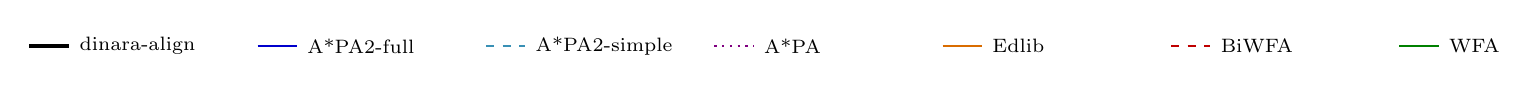
\begin{tikzpicture}[font=\scriptsize]
\draw[dinara] (0.00,0) -- (0.50,0) node[right,black] {dinara-align};
\draw[apafull] (2.90,0) -- (3.40,0) node[right,black] {A*PA2-full};
\draw[apasimple] (5.80,0) -- (6.30,0) node[right,black] {A*PA2-simple};
\draw[apa] (8.70,0) -- (9.20,0) node[right,black] {A*PA};
\draw[edlib] (11.60,0) -- (12.10,0) node[right,black] {Edlib};
\draw[biwfa] (14.50,0) -- (15.00,0) node[right,black] {BiWFA};
\draw[wfa] (17.40,0) -- (17.90,0) node[right,black] {WFA};
\end{tikzpicture}}
\caption{Unit-cost alignment of uniform pairs, mean time per alignment on a logarithmic scale. (a) 100~kbp pairs by divergence; dinara-align had the lowest mean time at every divergence except 10\%. (b) Pairs at 15\% divergence by length; lines end where a tool completed no pair within 20~s, and hollow points mark tools that completed only some pairs.}\label{fig:sweeps}
\end{figure*}

On the ultra-long reads, an alignment increased peak memory by 51~MB without and 37~MB with genetic variation, compared with 81 and 48~MB for A*PA2-full and 82 and 32~MB for A*PA2-simple; on 1~Mbp pairs at 15\% divergence, by 55~MB, compared with 86 to 149~MB for A*PA and A*PA2. On shorter inputs dinara-align generally used more memory than the most economical tool, for example 13~MB against 2.3~MB for Edlib on 300~kbp pairs at 5\% divergence, and its runtime occupies about 13~MB, compared with 3 to 5~MB for the other tools.

\subsection{Gap-affine costs, other modes and batches}

At the WFA costs (4, 6, 2), dinara-align was 1.7 to 3.2 times faster than WFA on every dataset that any tool completed, and was the only aligner to complete all 104 reads of the 50~kbp dataset within the time limit (Table~\ref{tab:affine}). In each of the 14 workloads covering local, overlap, infix, prefix, extension, two-piece and substitution-matrix alignment, it was faster than the fastest alternative, by factors from 1.1 to 10.6 (Supplementary Table S2).

\begin{table*}[t]
\caption{Gap-affine alignment at costs (4, 6, 2): mean time per alignment with a 5~s budget per sample. Superscripts give the number of pairs completed where not all were.}\label{tab:affine}
\centering\footnotesize
\setlength{\tabcolsep}{4pt}
\begin{tabular}{@{}lrrrr@{}}
\toprule
Dataset & dinara-align & WFA & BiWFA & KSW2 \\
\midrule
ont-1k & \textbf{112~\textmu s} & 186~\textmu s & 304~\textmu s & 1.1~ms \\
ont-10k & \textbf{1.68~ms} & 4.8~ms & 5.84~ms & 30.8~ms$^{163/277}$ \\
ont-50k & \textbf{21.2~ms} & 68.4~ms$^{82/104}$ & 57.3~ms$^{90/104}$ & 367~ms$^{16/104}$ \\
SARS-CoV-2 & \textbf{755~\textmu s} & 2.06~ms & 1.79~ms & 88.4~ms \\
10~kbp, 5\% & \textbf{2.17~ms} & 6.36~ms & 8.02~ms & 97.1~ms$^{52/99}$ \\
10~kbp, 15\% & \textbf{12.2~ms} & 38.5~ms & 44.8~ms & 203~ms$^{25/99}$ \\
\bottomrule
\end{tabular}
\end{table*}

Following the short-read case study of Accelign \citep{Kallenborn2026accelign}, we computed global scores for 500{,}000 pairs of 148~bp reads with 1\% error against reference segments of similar length (Table~\ref{tab:batch}). Under gap-affine costs (mismatch 1, gap \(2+k\)), dinara-align required 0.47~\textmu s per pair on one core, compared with 2.12~\textmu s for WFA2-lib, and 26~ms for the whole batch on ten cores, compared with 115~ms.

\begin{table*}[t]
\caption{Global scores of 500{,}000 short-read pairs; each time is the whole call.}\label{tab:batch}
\centering\footnotesize
\setlength{\tabcolsep}{4pt}
\begin{tabular}{@{}llrrrrr@{}}
\toprule
Costs & Threads & dinara-align & WFA2-lib & KSW2 & parasail & Edlib \\
\midrule
Affine (1, 2, 1) & 1 & \textbf{233~ms} & 1.06~s & 10.9~s & 21.7~s & – \\
Unit & 1 & \textbf{212~ms} & 450~ms & – & – & 2.0~s \\
Affine (1, 2, 1) & 10 & \textbf{26~ms} & 115~ms & 1.18~s & 2.34~s & – \\
Unit & 10 & \textbf{26~ms} & 48~ms & – & – & 223~ms \\
\bottomrule
\end{tabular}
\end{table*}

\subsection{Effect of each technique}

To measure what each technique contributes, dinara-align was built with one technique switched off at a time, everything else unchanged, and every build aligned the A*PA2 samples with traceback and scored the short-read batch. The builds alternated within each of three rounds, pinned to one core, and we report the median against the build with every technique on (Table~\ref{tab:ablation}). Because the Skylake-X penalises jumps that cross 32-byte boundaries, the position of a loop after a rebuild can move the running time by several percent; the alignment builds were therefore assembled with branches kept clear of those boundaries (\texttt{-mbranches-within-32B-boundaries}). A baseline built in this way from a different source file ran within 0.7\% of the baseline on every dataset, the baseline varied by at most 1.2\% between rounds, and every build returned the same costs on every dataset. Constructing the neighbours of exact seed matches directly contributed most on long, divergent pairs: without it, the ultra-long reads took 9\% and 16\% longer and the 100~kbp pairs at 10 and 15\% divergence 9 to 10\% longer. Interleaving two groups of bit-parallel words contributed 4 to 5\% on the ultra-long reads, over this and a second, independent set of builds; the regrouped recurrence, although it shortens a single word's step from 14 to 8 cycles, contributed 1 to 2\%, because bands narrow enough to be bound by that step make up a small part of the work. Gathered diagonal transition contributed 13 to 24\% where diagonal transition does most of the work, on the 1~kbp reads, the SARS-CoV-2 genomes and near-identical 100~kbp pairs. The agreement rule for extrapolated bounds mattered on the 10~kbp reads (18\%) and the SARS-CoV-2 genomes (6\%), and not on the ultra-long reads, where the seed heuristic sets the first bound. Without the certified band, the short-read batch took 2.9 and 3.1 times as long at affine and unit costs.

\begin{table*}[t]
\caption{Effect of each technique: median time with all techniques on (ms per alignment; per batch of 500{,}000 pairs for the short reads), and the change when one technique is switched off, over three alternating rounds on the Skylake-X, with branches kept clear of 32-byte boundaries. Every configuration returned the same costs.}\label{tab:ablation}
\centering\footnotesize
\setlength{\tabcolsep}{4pt}
\begin{tabular}{@{}lrrrrrrr@{}}
\toprule
Dataset & All on & Regrouped recurrence & Paired groups & Gathers & Agreement rule & Seed neighbours & Certified band \\
\midrule
ont-500k & 96.5 & +0.9\% & \textbf{+4.3\%} & −0.1\% & −0.3\% & \textbf{+9.0\%} &  \\
ont-500k-genvar & 134.1 & +1.1\% & \textbf{+4.2\%} & −0.1\% & −0.2\% & \textbf{+16.0\%} &  \\
ont-1k & 0.021 & −0.4\% & −0.5\% & \textbf{+14.1\%} & −0.4\% & −0.3\% &  \\
ont-10k & 0.151 & −1.3\% & +0.9\% & +3.5\% & \textbf{+17.5\%} & +0.1\% &  \\
SARS-CoV-2 & 0.195 & −0.5\% & +0.2\% & \textbf{+13.1\%} & \textbf{+5.5\%} & +0.3\% &  \\
100~kbp, 1\% & 0.971 & −0.4\% & 0.0\% & \textbf{+24.2\%} & −0.1\% & +0.1\% &  \\
100~kbp, 5\% & 4.39 & −0.3\% & −0.6\% & −0.2\% & +0.1\% & −0.6\% &  \\
100~kbp, 10\% & 10.1 & −0.7\% & −0.2\% & +0.8\% & +0.1\% & \textbf{+10.4\%} &  \\
100~kbp, 15\% & 10.65 & 0.0\% & +1.1\% & +2.4\% & +0.3\% & \textbf{+9.4\%} &  \\
Short reads, affine & 232 &  &  &  &  &  & \textbf{+187\%} \\
Short reads, unit & 212 &  &  &  &  &  & \textbf{+214\%} \\
\bottomrule
\end{tabular}
\end{table*}

\section{Discussion}

The algorithms in dinara-align build on those of earlier exact aligners; the gains come from changes to how these algorithms use the processor. Two observations stand out. First, on long pairs the techniques that reduce work outside the inner loop contributed more than those that speed it up: constructing seed neighbours directly saved up to 16\%, against 4 to 5\% for interleaving bit-parallel groups and 1 to 2\% for the regrouped recurrence (Table~\ref{tab:ablation}). Second, as the inner loops become faster, the scalar, memory-bound construction of the seed heuristic dominates: on 100~kbp pairs at 10\% divergence it accounts for 58\% of the running time and is the main cost in the one configuration in which A*PA2-full remained faster. Neither the regrouped recurrence nor the per-lane band certificate depends on the implementation, and both apply directly to other bit-parallel and inter-sequence aligners.

The study has several limitations. First, the evaluation covers a single x86 processor with AVX-512. The AVX2 configuration was measured only for its inexact-seed threshold, built for Haswell on the same machine (20 and 30\% equal within 0.5\%, 40\% up to 6\% slower), and the NEON configuration, which the library also supports, is not evaluated here. Second, some thresholds were chosen using workloads that also appear in the evaluation; in particular, the AVX-512 threshold for inexact seeds was lowered from 40 to 20\% after measurements on the uniform 100~kbp pairs of Fig.~\ref{fig:sweeps}a, so results on those pairs may overstate performance on unseen data. Third, as in the A*PA2 protocol, most configurations were run once, and on the Skylake-X some running times varied by up to one third between builds that did not change the code involved, which we attribute to code alignment effects in the instruction decoder; the ablation controls for this, the comparison with other tools does not. Fourth, the ablation switches off one technique at a time against the full configuration, so it does not separate interactions between techniques. Finally, release builds target the baseline processor of each platform, so the AVX-512 code paths require a build for the host processor.

Future work includes speeding up seed construction, reusing computation across band-doubling rounds as in the incremental doubling of A*PA2, measurements on further processors, and GPU implementations of the same algorithms.

\section*{Funding}
This work received no specific funding.

\section*{Conflict of interest}
None declared.

\section*{Data availability}
The software, benchmark harness and the commits of every compared tool are available at \url{https://github.com/kokyriakidis/dinara-align}. The benchmarks are reproduced by \texttt{pixi run bench-astarpa2}, \texttt{results-astarpa2}, \texttt{bench}, \texttt{bench-local}, \texttt{bench-modes}, \texttt{bench-batch} and \texttt{bench-ablation}.

\bibliographystyle{plainnat}
\bibliography{references}
\end{document}
